\section{Resultados Experimentais}
\label{sec:resultados_experimentais}

A validação experimental do sistema de navegação autônoma desenvolvido para a plataforma VIDA foi realizada por meio de ensaios em ambiente real, buscando avaliar a integração dos subsistemas de sensoriamento, estimação de estados, controle de baixo nível e seguimento de trajetórias. Os experimentos permitiram verificar o funcionamento da arquitetura computacional distribuída e avaliar o comportamento do veículo durante a execução autônoma de percursos previamente definidos.

Foram realizados dois experimentos de seguimento autônomo de trajetória, denominados Trajeto 1 e Trajeto 2. A avaliação foi conduzida a partir dos dados registrados pelo ROS~2, considerando as trajetórias de referência e executadas, os erros de seguimento, os comandos de controle e as informações disponibilizadas pelo estimador de estados.

\subsection{Procedimento Experimental}
\label{subsec:procedimento_experimental}

Os ensaios foram realizados com a plataforma VIDA, utilizando os subsistemas de controle, localização e navegação apresentados nos capítulos anteriores.

As trajetórias de referência foram obtidas a partir de coordenadas geográficas registradas pelo receptor GNSS durante a condução manual do veículo. Os pontos coletados foram posteriormente processados por meio de suavização e reamostragem, resultando em trajetórias com espaçamento uniforme de 0,25~m, armazenadas em arquivos CSV e utilizadas pelo sistema de navegação autônoma.

O desempenho dos controladores de baixo nível foi avaliado pela comparação entre as referências de velocidade longitudinal e ângulo de esterçamento e as respectivas respostas medidas durante os ensaios.

Em ambos os experimentos, foi utilizada uma referência de velocidade longitudinal de 2,0~m/s. Para a avaliação quantitativa do desempenho do seguimento, foram considerados o erro médio absoluto (MAE), o erro quadrático médio (RMSE) e o erro máximo absoluto, calculados a partir dos erros laterais registrados durante a navegação autônoma.

em que $e_i$ representa o erro lateral registrado em cada amostra e $N$ corresponde ao número total de amostras consideradas. O erro máximo absoluto corresponde ao maior valor de $|e_i|$ observado durante cada experimento.

\subsection{Desempenho dos Controladores de Baixo Nível}
\label{subsec:resultados_baixo_nivel}

Os resultados experimentais dos controladores de baixo nível são apresentados a seguir, iniciando pela malha de esterçamento e, posteriormente, pela malha de velocidade longitudinal.

O controlador PID de esterçamento apresentou capacidade de acompanhar as referências angulares fornecidas pelo controlador Stanley durante o seguimento autônomo de trajetória. Conforme apresentado na Figura~\ref{fig:resposta_esterçamento}, o ângulo medido pelo sensor LVDT acompanhou as variações da referência, apresentando erro quadrático médio (RMS) de 1,68° e atraso estimado de aproximadamente 175~ms.

Ao compensar esse atraso na análise dos sinais, o erro RMS foi reduzido para 0,68°, indicando que a defasagem temporal representa uma parcela significativa do erro observado. O erro máximo absoluto registrado foi de 4,47°, observado após uma curva mais fechada à direita, quando a referência de esterçamento variou rapidamente de aproximadamente 20° para -20°.

Observa-se também que a resposta apresenta pequenos movimentos em degraus, especialmente durante variações reduzidas da referência. Esse comportamento é compatível com a zona morta de atuação implementada no controlador, cuja finalidade é evitar acionamentos repetitivos do mecanismo de direção diante de pequenas variações do erro.

\begin{figure}[htb]
    \centering
    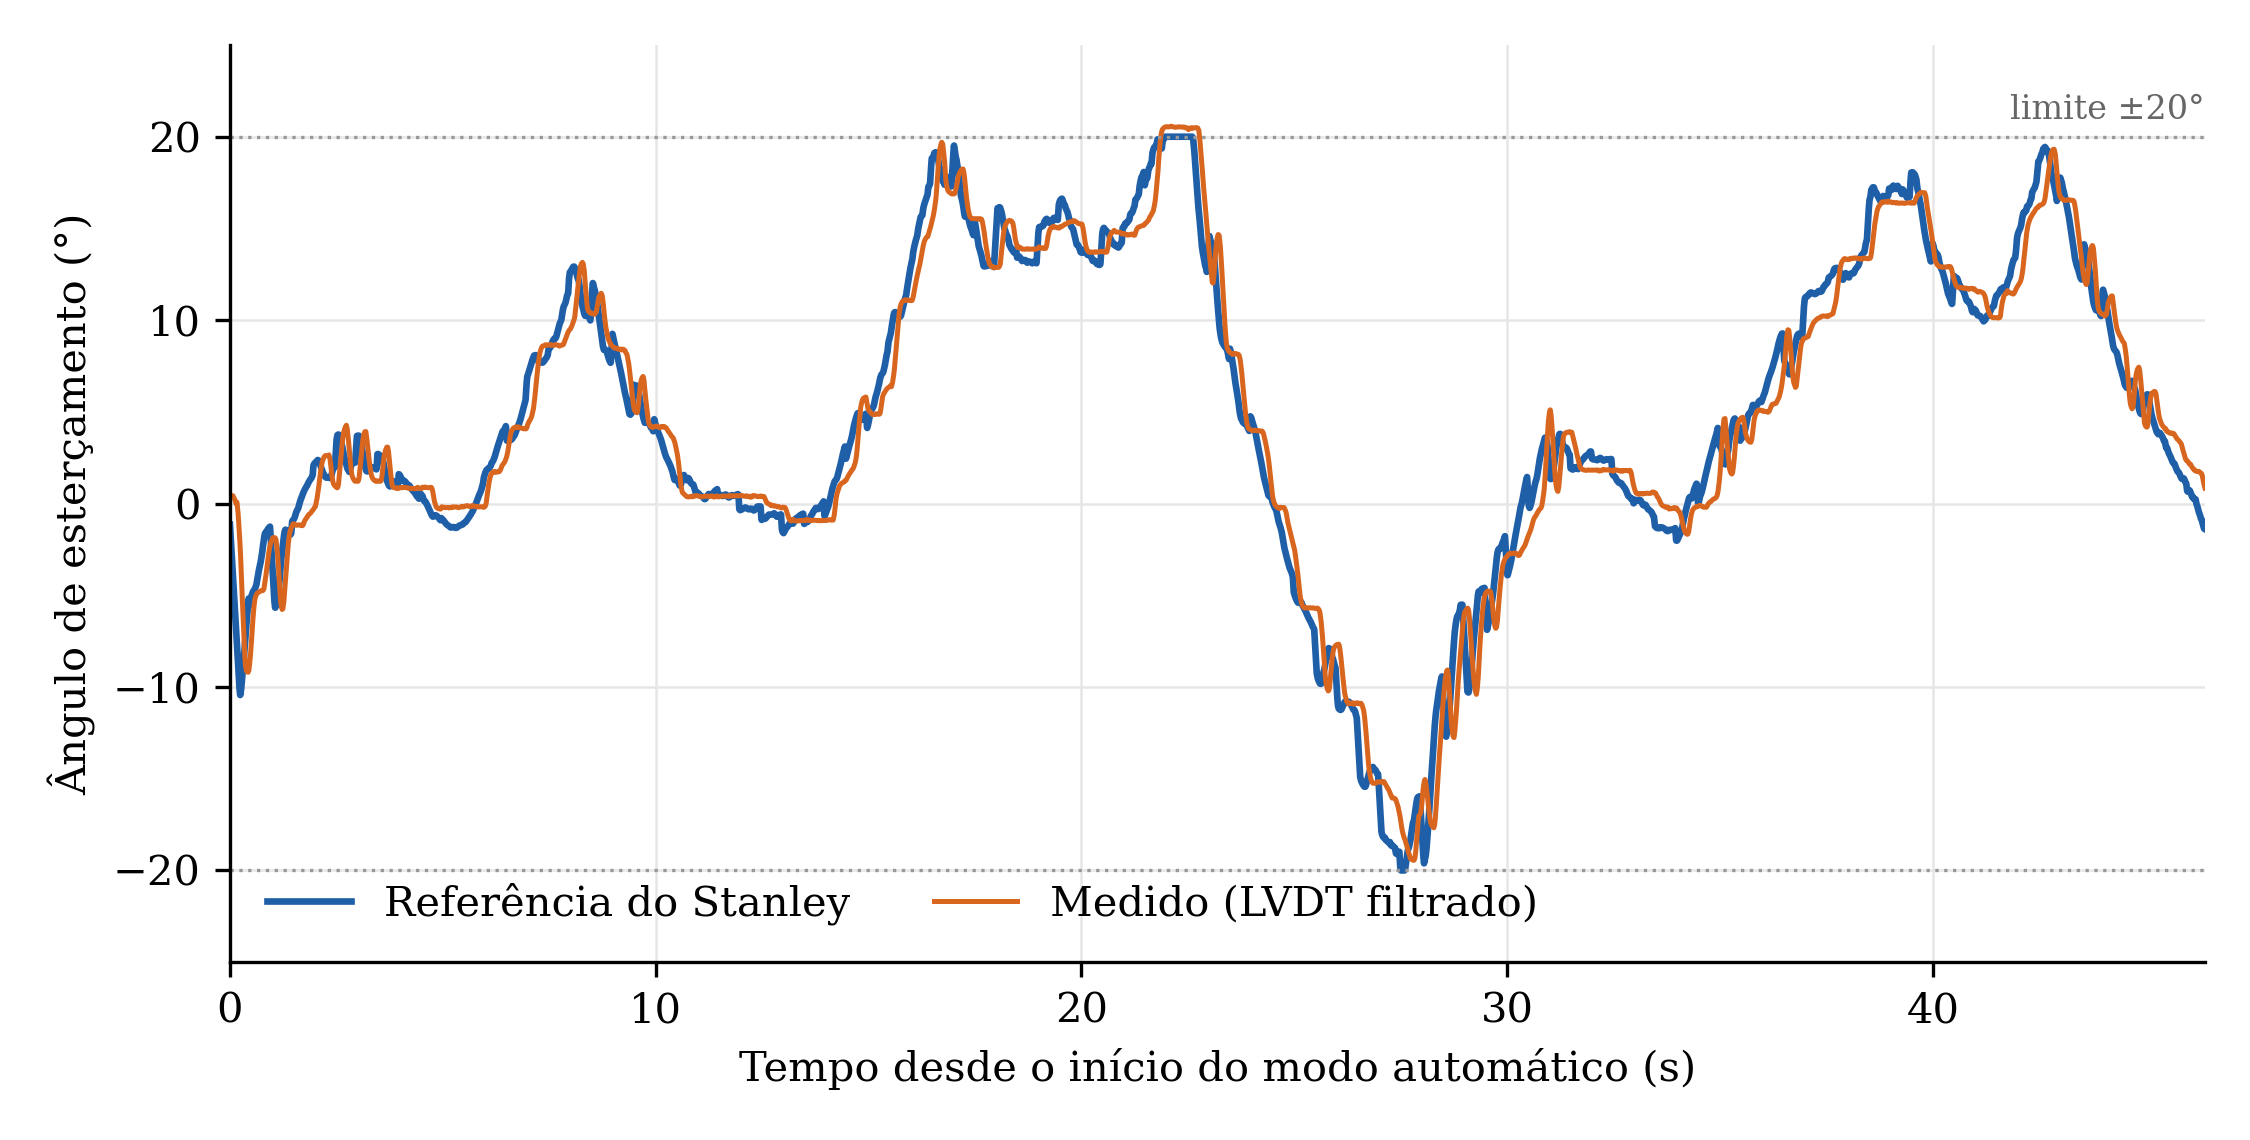
\includegraphics[width=\columnwidth]{Imagens/Resposta PID esterçamento.png}
    \caption{Resposta experimental do controlador de esterçamento. Fonte: Elaborado pelo autor.}
    \label{fig:resposta_esterçamento}
\end{figure}

O controlador PI de velocidade longitudinal foi avaliado quanto à capacidade de manter a velocidade do veículo próxima à referência de 2,0~m/s durante o seguimento autônomo de trajetória. Conforme apresentado na Figura~\ref{fig:resposta_velocidade}, a velocidade medida apresentou pequenas oscilações em torno da referência. Considerando o regime permanente, a velocidade média foi de 1,998~m/s, com erro quadrático médio (RMS) de 0,063~m/s, equivalente a aproximadamente 3,1\% da referência. O erro máximo absoluto registrado foi de 0,187~m/s.

As oscilações observadas estão relacionadas à zona morta de acionamento do motor, que exige um sinal PWM mínimo de aproximadamente 7,8\% para produzir esforço suficiente. Entretanto, o esforço necessário para manter a velocidade de referência corresponde a aproximadamente 6,5\% do PWM. Dessa forma, o menor acionamento disponível produz uma aceleração superior à necessária, fazendo com que a velocidade ultrapasse a referência. O controlador PI então interrompe a tração, permitindo que o veículo desacelere naturalmente devido às resistências ao movimento. Quando a velocidade retorna a valores inferiores à referência, a tração é restabelecida, produzindo oscilações periódicas em torno da velocidade desejada.

\begin{figure}[htb]
    \centering
    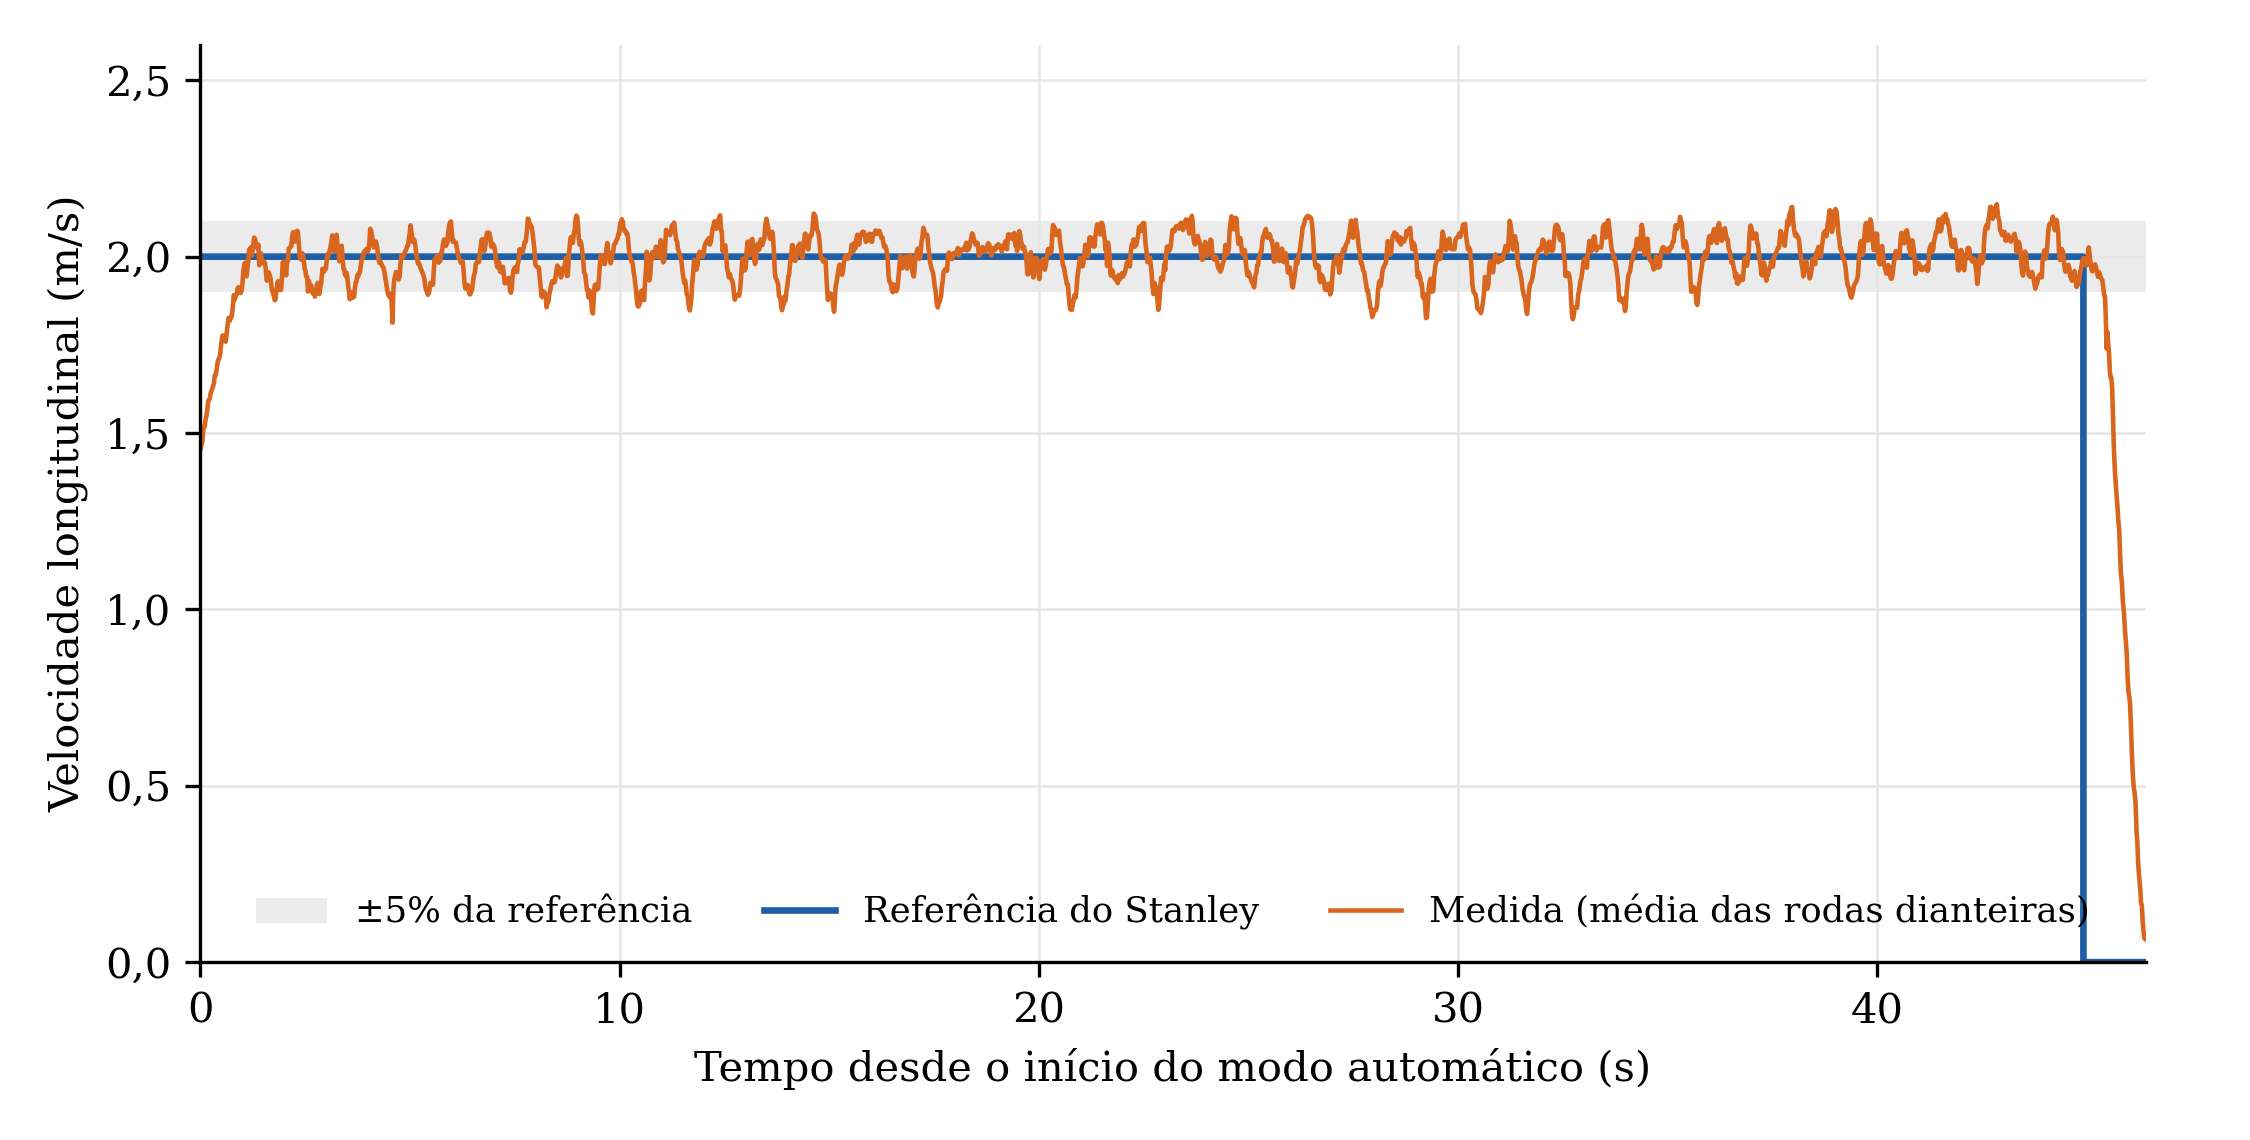
\includegraphics[width=0.96\columnwidth]{Imagens/Resposta PI velocidadade longitudinal.png}
    \caption{Resposta experimental do controlador de velocidade longitudinal. Fonte: Elaborado pelo autor.}
    \label{fig:resposta_velocidade}
\end{figure}

Apesar dessas oscilações, o controlador apresentou desempenho satisfatório na manutenção da velocidade longitudinal. Durante o regime permanente, o veículo permaneceu 88,6\% do tempo dentro de uma faixa de tolerância de $\pm 5\%$ em relação à referência e 100\% do tempo dentro de $\pm 10\%$. Esse comportamento é favorecido pela inércia do veículo, que suaviza as variações de velocidade provocadas pelos acionamentos intermitentes do motor de tração.


\subsection{Seguimento de Trajetória: Trajeto 1}

O primeiro ensaio de seguimento autônomo de trajetória foi realizado em um estacionamento localizado nas proximidades do Departamento de Engenharia de Alimentos da Universidade Federal de Lavras (UFLA). O local apresenta uma área aberta, favorável à recepção dos sinais GNSS e à realização dos experimentos com a plataforma VIDA.

A trajetória de referência foi obtida por meio da condução manual do veículo ao longo do percurso estabelecido, durante a qual foram registradas as coordenadas geográficas fornecidas pelo receptor GNSS. Posteriormente, esses pontos foram utilizados como referência para o seguimento autônomo de trajetória pelo controlador Stanley.

Durante o ensaio, o veículo percorreu aproximadamente 88~m em modo automático, ao longo de 46,4~s, mantendo velocidade média de 1,97~m/s, próxima à referência de 2,0~m/s. A Figura~\ref{fig:trajeto_1} apresenta a comparação entre a trajetória de referência e o percurso realizado pelo veículo.


\begin{figure}[htb]
    \centering
    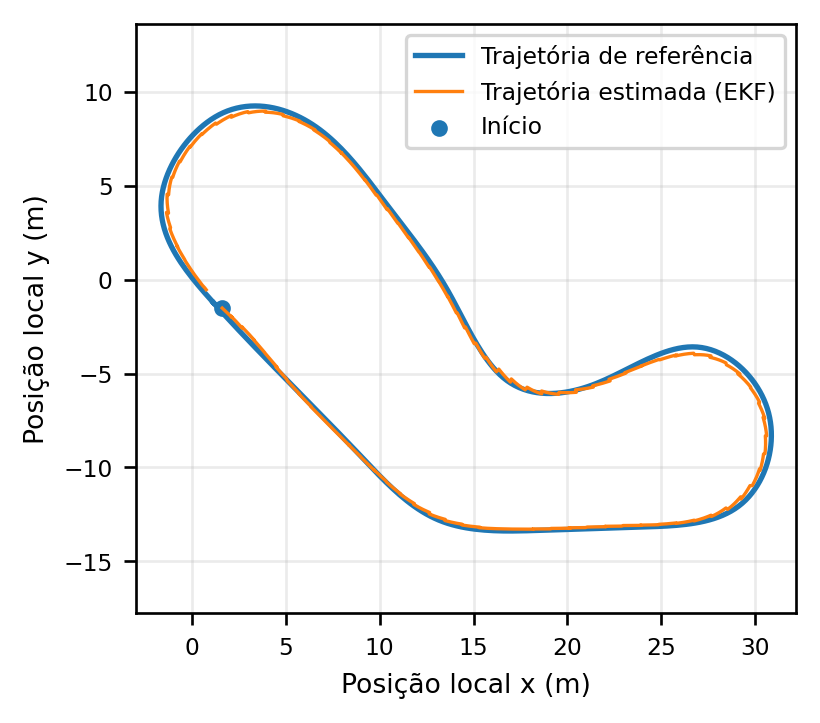
\includegraphics[width=0.85\columnwidth]{Imagens/Trajetoria_Troia.png}
    \caption{Comparação entre a trajetória de referência e a trajetória percorrida pelo veículo no Trajeto 1. Elaborado pelo autor.}
    \label{fig:trajeto_1}
\end{figure}

A avaliação do desempenho do controlador Stanley foi realizada a partir do erro lateral de seguimento. A Figura~\ref{fig:erro_lateral_trajeto_1} apresenta a evolução desse erro durante o percurso.

\begin{figure}[htb]
    \centering
    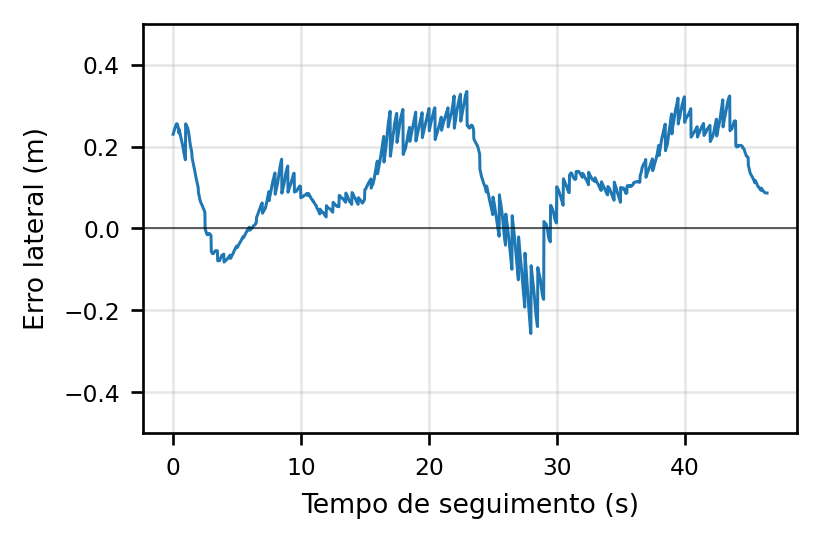
\includegraphics[width=0.85\columnwidth]{Imagens/Erro_Lateral_Troia.png}
    \caption{Evolução do erro lateral de seguimento durante o Trajeto 1.Elaborado pelo autor.}
    \label{fig:erro_lateral_trajeto_1}
\end{figure}

O testez, o erro lateral apresentou valor quadrático médio (RMS) de 0,167~m e valor máximo absoluto de 0,33~m.

Os resultados indicam que o controlador Stanley foi capaz de conduzir a plataforma VIDA ao longo da trajetória estabelecida, mantendo desvios laterais relativamente pequenos durante o percurso. Dessa forma, o ensaio demonstrou o funcionamento integrado dos sistemas de localização, navegação e controle no seguimento autônomo de trajetória.



\subsection{Seguimento de Trajetória: Trajeto 2}
\label{subsec:trajeto_2}

O segundo ensaio de seguimento autônomo de trajetória foi realizado no autódromo da Universidade Federal de Lavras (UFLA), utilizando um percurso mais extenso e com diferentes características geométricas em relação ao primeiro experimento. A trajetória apresenta curvas e mudanças de direção, permitindo avaliar o desempenho do controlador Stanley durante a execução de manobras sucessivas.

\begin{figure}[htb]
    \centering
    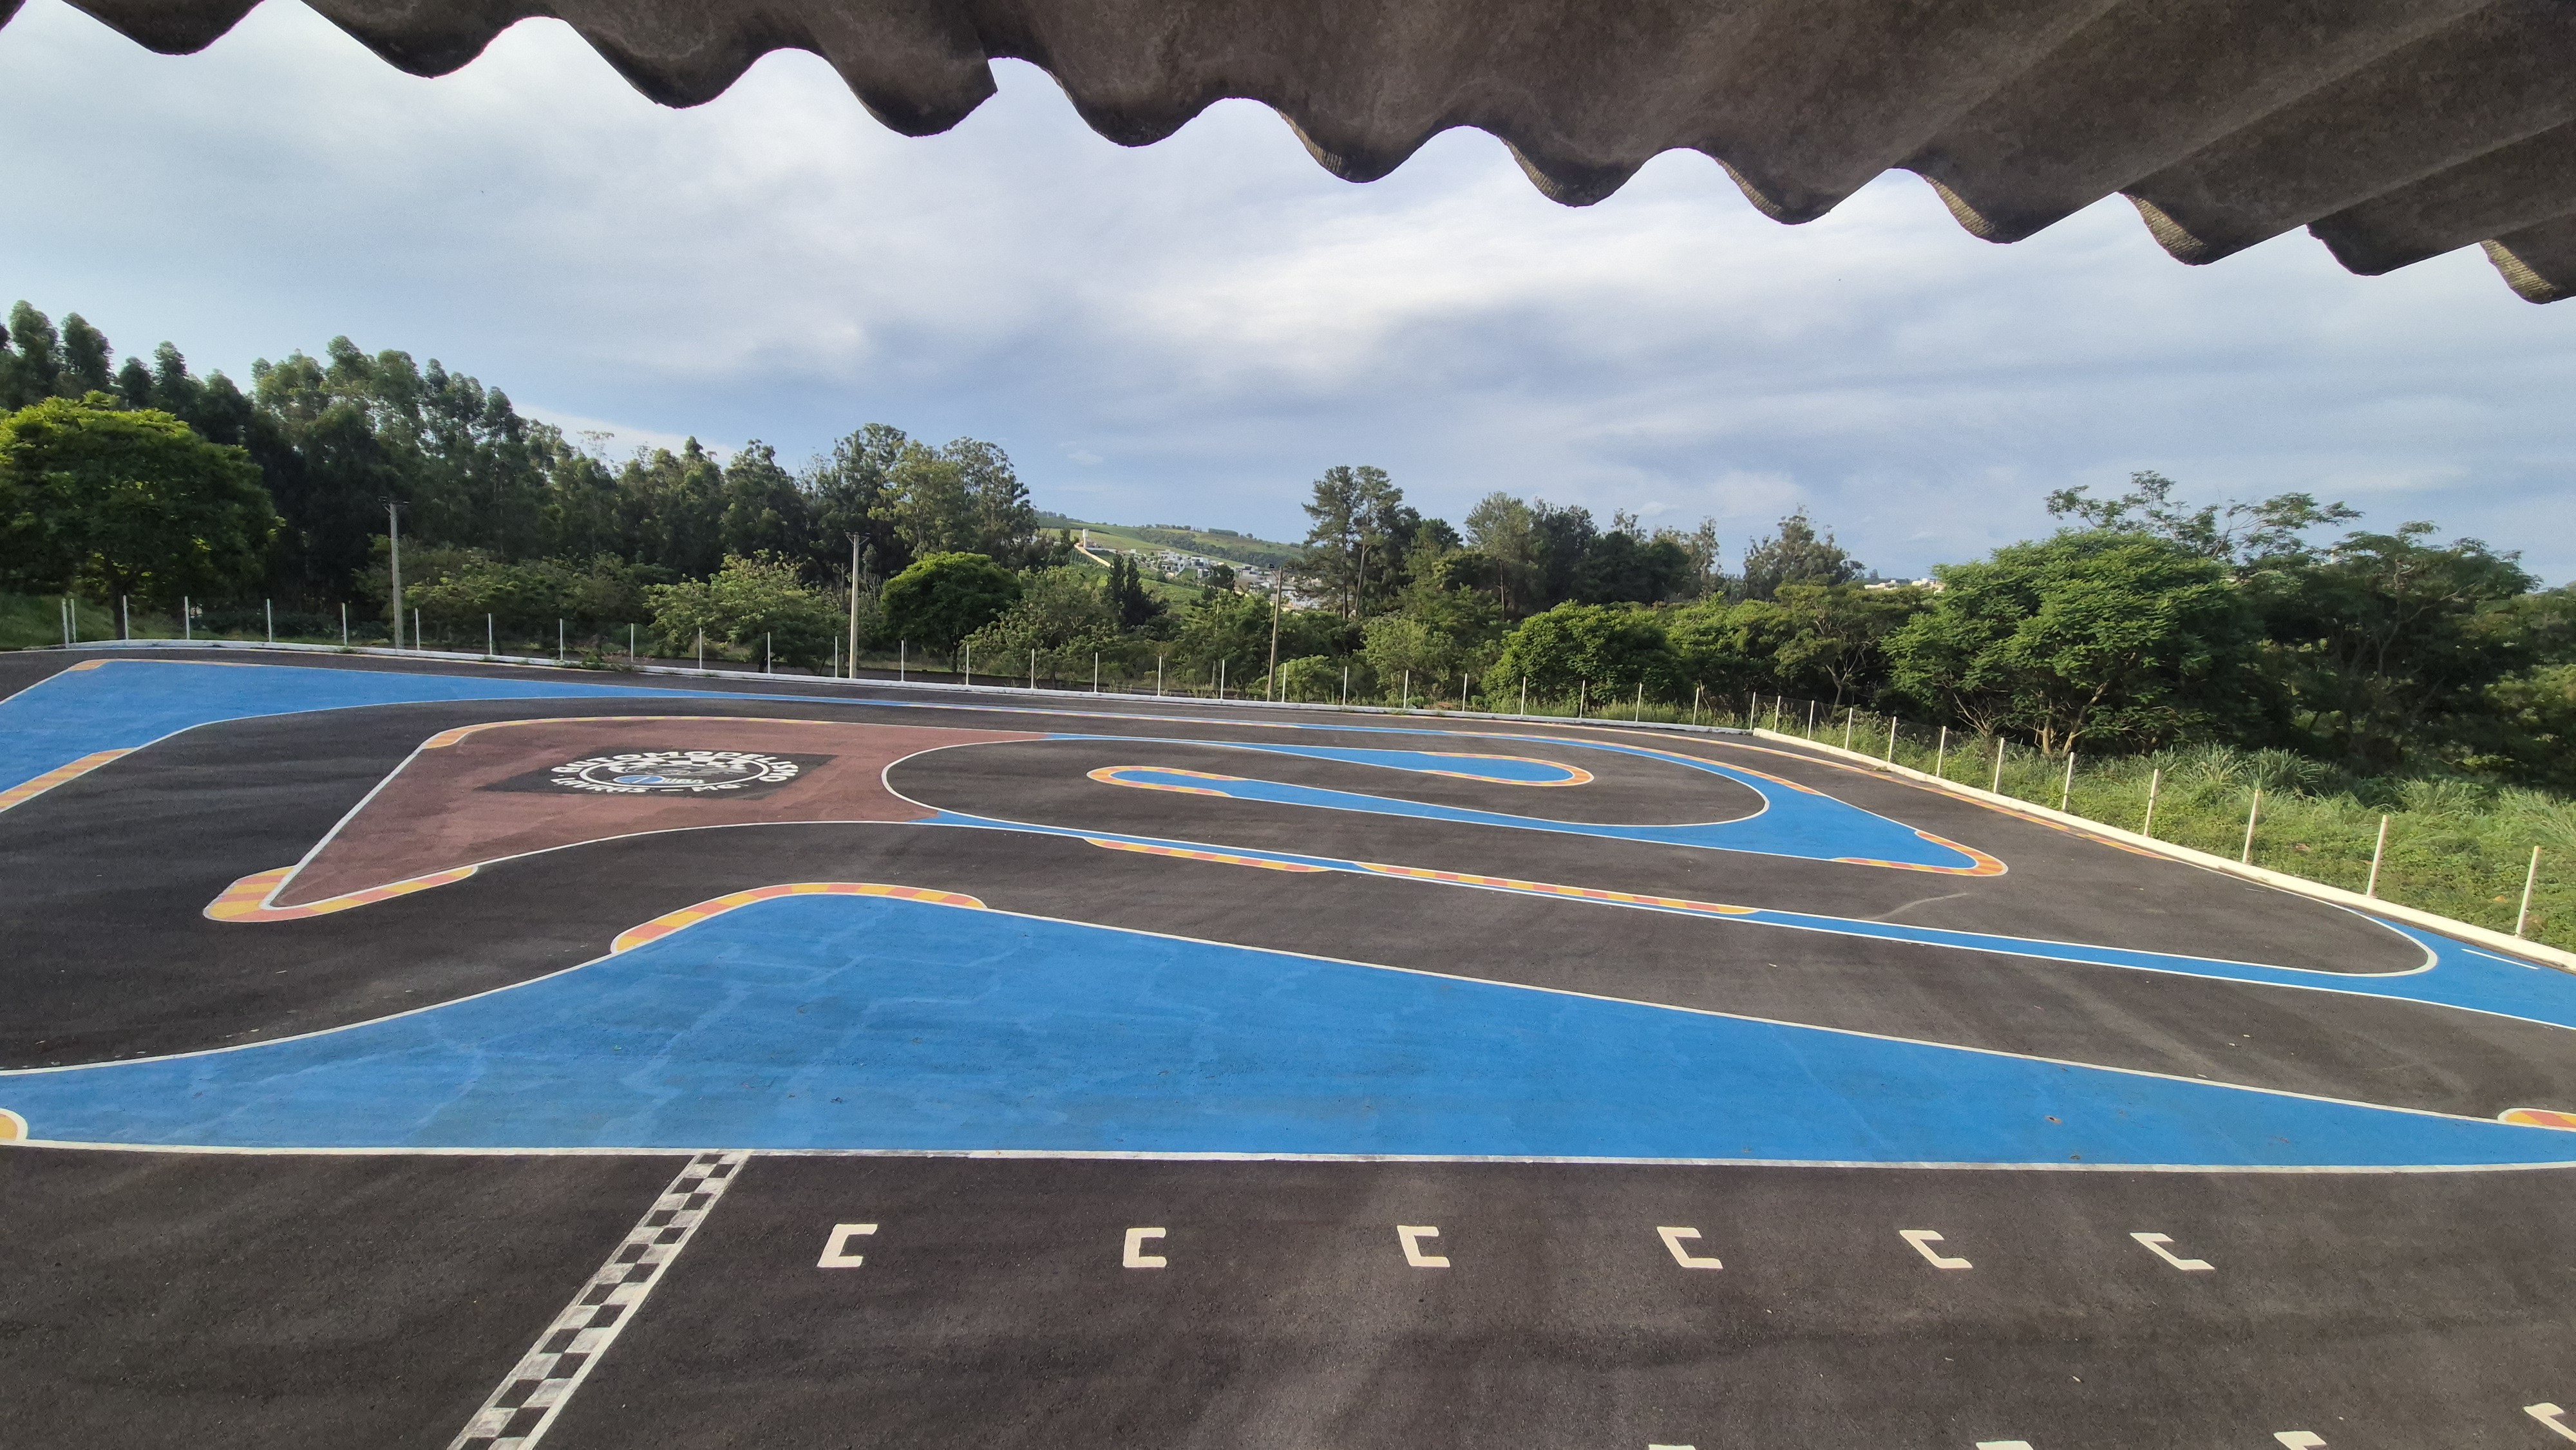
\includegraphics[width=0.85\columnwidth]{Imagens/Autodromo_UFLA.jpg}
    \caption{Vista geral do autódromo da Universidade Federal de Lavras, utilizado no ensaio de seguimento autônomo de trajetória do Trajeto 2. Fonte: Acervo pelo autor.}
    \label{fig:pista_trajeto_2}
    
\end{figure}

A trajetória de referência foi previamente registrada e posteriormente utilizada pelo sistema de navegação para a execução do percurso em modo autônomo. Durante o ensaio, o veículo percorreu aproximadamente 281,42~m ao longo de 146,56~s, utilizando uma velocidade de referência de 2,0~m/s.

A Figura~\ref{fig:trajeto_2} apresenta a comparação entre a trajetória de referência e o percurso realizado pelo veículo durante o experimento.

\begin{figure}[htb]
    \centering
    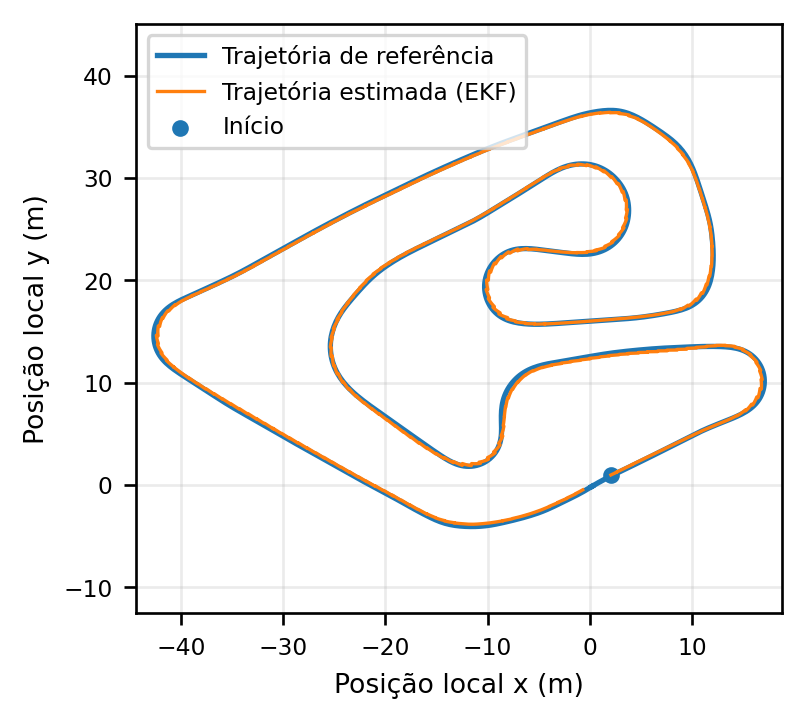
\includegraphics[width=0.85\columnwidth]{Imagens/Trajetoria_Pista3.png}
    \caption{Comparação entre a trajetória de referência e a trajetória percorrida pelo veículo no Trajeto 2. Elaborado pelo autor.}
    \label{fig:trajeto_2}
    
\end{figure}

Observa-se que o veículo foi capaz de acompanhar a trajetória estabelecida ao longo do percurso, realizando as correções de esterçamento necessárias para compensar os desvios laterais e de orientação. A execução desse experimento é particularmente relevante por envolver um trajeto mais extenso, exigindo a atuação contínua do controlador durante diferentes condições de curvatura.

A Figura~\ref{fig:erro_lateral_trajeto_2} apresenta a evolução temporal do erro lateral de seguimento durante o ensaio.

\begin{figure}[htb]
    \centering
    \includegraphics[width=0.85\columnwidth]{Imagens/erro_lateral_Pista3.png}
    \caption{Evolução do erro lateral de seguimento durante o Trajeto 2. Elaborado pelo autor.}
    \label{fig:erro_lateral_trajeto_2}
\end{figure}

Durante o experimento, o erro lateral médio absoluto (MAE) foi de 0,108~m, enquanto o erro quadrático médio (RMSE) apresentou valor de 0,129~m. O maior erro absoluto registrado foi de aproximadamente 0,366~m.

Esses resultados demonstram que o controlador Stanley foi capaz de manter o veículo próximo à trajetória de referência, mesmo diante das diferentes condições geométricas do percurso. Ao final do trajeto, o sistema de navegação identificou a conclusão da trajetória e realizou a transição para a condição de parada, evidenciando o funcionamento integrado dos sistemas de localização, navegação e controle da plataforma VIDA.

\subsection{Análise Comparativa dos Experimentos}

Os resultados quantitativos obtidos nos dois experimentos são apresentados na Tabela~\ref{tab:resultados_seguimento}. As métricas correspondem aos períodos de navegação autônoma identificados nos registros experimentais.

\begin{table}[htb]
    \centering
    \caption{Resultados experimentais do seguimento autônomo de trajetórias.}
    \label{tab:resultados_seguimento}
    \begin{tabular}{lcc}
        \hline
        \textbf{Métrica} & \textbf{Troia} & \textbf{Pista 3} \\
        \hline
        Percurso (m) & 89,24 & 281,42 \\
        Duração (s) & 46,48 & 146,56 \\
        MAE lateral (m) & 0,143 & 0,108 \\
        RMSE lateral (m) & 0,167 & 0,129 \\
        Erro máximo (m) & 0,334 & 0,366 \\
        Velocidade ref. (m/s) & 2,0 & 2,0 \\
        \hline
    \end{tabular}
\end{table}

A comparação demonstra que o sistema foi capaz de executar autonomamente dois percursos com diferentes comprimentos e características geométricas. O segundo experimento apresentou um comprimento de referência aproximadamente 3,15 vezes superior ao primeiro, mantendo valores reduzidos de erro lateral ao longo da execução.

Na Pista Troia, o RMSE lateral foi de 0,167 m, enquanto na Pista 3 foi de 0,129 m, representando uma redução aproximada de 22,8\% no erro quadrático médio. De maneira semelhante, o MAE lateral diminuiu de 0,143 m para 0,108 m.

Entretanto, essa diferença não deve ser interpretada isoladamente como uma melhoria intrínseca do controlador, uma vez que os experimentos foram realizados em trajetórias distintas e podem apresentar diferenças de geometria, condições de superfície, alinhamento inicial e qualidade das estimativas de localização.

De modo geral, os resultados indicam que a implementação do controlador Stanley, associada ao sistema de estimação de estados e aos controladores de baixo nível, possibilitou o seguimento autônomo das trajetórias avaliadas. A execução dos percursos também demonstrou a viabilidade da arquitetura distribuída implementada, permitindo integrar os diferentes subsistemas necessários à navegação autônoma do VIDA.

É importante destacar que as métricas de erro lateral foram calculadas a partir das estimativas utilizadas pelo próprio sistema de navegação. Dessa forma, representam o desempenho de seguimento avaliado no referencial do controlador, não constituindo uma medição independente da trajetória física efetivamente percorrida.

Apesar dessa limitação, os experimentos representam uma validação funcional do sistema desenvolvido, demonstrando a execução de trajetórias autônomas com erros laterais quadráticos médios inferiores a 0,17 m nas condições avaliadas. Os resultados fornecem uma base experimental para futuros aprimoramentos dos algoritmos de localização, controle e planejamento de trajetórias da plataforma VIDA.
